
%% Author: Egill B�i Einarsson
%% PTG, Parsing Table Generator
%% See copyleft below or in the generated document.

\documentclass[11pt,a4paper]{article}

\usepackage[american]{babel}
\usepackage[pdftex]{hyperref}
\usepackage{times}
\usepackage{float}
\usepackage[T1]{fontenc}
\usepackage[margin=1in]{geometry}
\usepackage{amsmath}
\usepackage{listings}
\usepackage{graphicx}
\usepackage{framed}
\usepackage{tikz}
\usetikzlibrary{arrows,automata}
\usetikzlibrary{shapes.multipart}
\usetikzlibrary{shapes.misc}

\begin{document}

\renewcommand{\contentsname}%
	{Table of Contents}
\renewcommand{\abstractname}%
	{abstract}
\sloppy
\title{PTG User Manual}
\author{Egill B�i Einarsson}
\maketitle

\begin{abstract}
PTG is a command-line program that generates files containing parsing tables and state machines for a formal language defined by an input grammar. Generated tables are in either \LaTeX{} or HTML format which eases automated inserting of generated elements. Likewise the state machines can be inserted directly when the TIKZ format is used. Alternativily state machines can use Graphviz's digraph automaton format which is intended for use with Graphviz DOT.
\end{abstract}

\section{Copyleft}
This program is free software: you can redistribute it and/or modify
it under the terms of the GNU General Public License as published by
the Free Software Foundation, either version 3 of the License, or
(at your option) any later version.


This program is distributed in the hope that it will be useful,
but WITHOUT ANY WARRANTY; without even the implied warranty of
MERCHANTABILITY or FITNESS FOR A PARTICULAR PURPOSE.  See the
GNU General Public License for more details.


You should have received a copy of the GNU General Public License
along with this program.  If not, see <http://www.gnu.org/licenses/>.

\tableofcontents

\section{Introduction}

PTG is run from a command-line terminal and generates parsing tables and state machines for context insensitive formal grammars. A grammar's FIRST, FOLLOW, LL(1), SLR(1), LALR(1) and LR(1) parsing tables can be generated in either \LaTeX{} or HTML format along with LR(0) and LR(1) state machines in Graphviz's digraph automaton format for use with DOT or TIKZ format for use directly in \LaTeX{}. The idea is when creating a document studying formal languages, that features some or all of these tables and machines, instead of writting theentites directly or copying a generated file into the master file PTG generated files can be dynamically linked in the master file. The result is that if the formal languages change then only the PTG grammar file needs to be updated, PTG run on the new grammar and Graphviz Dot on any digraph automaton format. The later two steps can of curse be automated with a make or batch file.

\section{Setup}

Setup is simple as long as a JRE(Java Runtime Environment) has been setup. Go to the \href{https://github.com/EgillEinarss/PTG}{PTG repository} on Github.com and download PTG.jar. Place this file in the current command line directory and run

\begin{lstlisting}[frame=single]
java -jar PTG.jar ...
\end{lstlisting}

\noindent along with any relevant arguments(detailed in the next section).

\subsection{Compiling the Source}

Required programs are \href{http://git-scm.com/}{git} and \href{http://www.gnu.org/software/make/}{make}.
Use a command line. If needed, go to your projects directory and get the project with the command

\begin{lstlisting}[frame=single]
git clone https://github.com/EgillEinarss/PTG.git
cd PTG
\end{lstlisting}

\noindent Alternatively go to the \href{https://github.com/EgillEinarss/PTG}{PTG repository} on Github.com and download what you want or require.
Now you have the developement environment setup that was used to create PTG. Now simply run the compilation process with the command

\begin{lstlisting}[frame=single]
make
\end{lstlisting}

\noindent Simple.
Feel free to modify the source code in the directory src, also any Java source files added into src will be compiled and added to the PTG jar file created by running make.


\section{Command Line Arguments}

The syntax for command line execution is:

\begin{lstlisting}[frame=single]
java -jar PTG.jar Grammar Options Output
\end{lstlisting}

\begin{description}
	\item[Grammar] The file containing the grammar to be parsed. Required and must be the first argument.
	\item[Options] A few options that define the grammar. Any number of them may be used and must be followed by a String, see Settings for String.
	\begin{description}
		\item[-START] Sets the grammar's start variable to String. Default is the first variable listed in Grammar.
		\item[-END] Sets the grammar's end of input token to String. Default is "\$".
		\item[-EMPTY] Sets the grammar's empty string token as String. Default is "<e>".
	\end{description}
	\item[Output] This is the output request. All of them can be followed by Settings, if a String is defined then it will be the output file name, the filename of the grammar is used as a default.
	\begin{description}
		\item[-ALL] Performs all of the following outputs.
		\item[-FIRST] Creates a First table.
		\item[-FOLLOW] Creates a Follow table.
		\item[-LL1] Creates a LL(1) table.
		\item[-SLR1] Creates a SLR(1) table.
		\item[-LR1] Creates a LR(1) table.
		\item[-LALR1] Creates a LALR(1) table.
		\item[-LR0M] Creates a LR(0) state machine.
		\item[-LR1M] Creates a LR(1) state machine.
		\item[-LALRM] Creates a LALR(0) state machine.
	\end{description}
	\item[Settings] Any and all settings are optional, some are not applicable but cause no error.
	\begin{description}
		\item[HTML] The table being defined will only have HTML output.
		\item[LATEX] The table being defined will only have \LaTeX output.
		\item[GZ] The state machine being defined will be in GraphViz's DOT format.
		\item[TIKZ] The state machine being defined will be in Tikz format.
		\item[TINY] The state machine being defined will contain only a label, will produce a table for more information.
		\item[SMALL] The state machine being defined will have a decreased description if possible.
		\item[LARGE] The state machine being defined will have a full description.
		\item[LR] The state machine being defined will go from left to right rather than top to bottom.
		\item[String] Any string of characters that is not one of the above defined keywords, pretty much anything is accepted but might cause catastrophic failure.
	\end{description}
\end{description}

Note that the keywords are in capital letters for clarity but in fact PTG is case insensitive in regards to keywords. Here are a few example calls:

\begin{lstlisting}[frame=single]
java -jar PTG.jar example.gra -all
java -jar PTG.jar filename -start Var2 -end EoF -empty e -ll1 html
\end{lstlisting}


\section{Preparing the Input Grammar File}

The Input Grammar File is a text file that contains the grammar to parse. There are no intended constraints on the filename or it's extension, the filename(that is without the dot and extension) will be used as a default prefix for any output filenames unless a new name is supplied by the input arguments. In the file each line is one rule, each rule contains a left-hand side, a seperator and a right-hand side in that order. The left-hand side and the seperator are one symbol each whereas the right-hand side is a string consisting of one or more symbols. A symbol is a whitespace terminated string of characters.

So a rule is a string of three or more symbols where the first is the left-hand side and the second is a seperator. PTG will interpret any left-hand side symbols as being a variable in the grammar and the left-hand side of the first rule is the default start variable. Any symbols in a right-hand side that is not a variable is a terminal symbol.

There is one special symbol which is the empty string symbol. In a rule that uses the empty symbol the right-hand side should consist of only the empty string symbol. The default empty string symbol is <e> but a new one can be defined as an input argument. To learn more about rules see \href{http://en.wikipedia.org/wiki/Formal_grammar#Context-free_grammars}{this Wikipedia article}.

Lastly a grammar is terminated by an empty line. This allows a comment to follow after the grammar for whatever reason. An example of a grammar is shown below, this example is used in the Example section below. Here the default start variable is S.

\begin{framed}
\lstinputlisting{examples/example.gra}
\end{framed}


\section{Implementing Generated Files}
\subsection{ \LaTeX{} Tables}
There are two simple ways to use generated \LaTeX{} tables, either by copy pasting or using the input command. PTG generates a tabular environment as opposed to an actual table environment, this is because a table (or other container, for example a figure) has commands that relate to placement of the environment in the document. The input command will allow the use of generated tex files directly. This allows a user to update a grammar file, run PTG for that grammar and then recompile the document. A table or figure environment can be used to contain the input command. Below is an example of how to insert a file named exampleTable.tex into a figure:

\begin{lstlisting}[frame=single]
\begin{table}
\centering
\input{exampleTable.tex}
\caption{A caption for the table}
\label{TableLabel}
\end{table}
\end{lstlisting}

Both the caption and label commands are optional and the arguments supplied for them are nonsense, $\backslash$centering is also optional.

\subsection{HTML Tables}

For now the recommendation is copy-pasting the contents of the generated file into the master file or just hyperlinking the generated file as an individual page from the master file. There should be a work-around with Javascript and it is quite simple to fix the problem with PHP.

\subsection{TIKZ Statemachines}

\begin{lstlisting}[frame=single]
\usepackage{tikz}
\usetikzlibrary{arrows,automata}
\usetikzlibrary{shapes.multipart}
\usetikzlibrary{shapes.misc}
\end{lstlisting}
Add these commands to the document header, between the documentclass and document directive, if missing. Now a generated Tikz statemachine contained in the file exampleMachine.tex can be added with:
\begin{lstlisting}[frame=single]
\input{exampleMachine.tex}
\end{lstlisting}


\subsection{Graphviz Statemachines}
Graphviz statemachine files have the extension .gz and should be rendered using Graphviz DOT. An example command to render exampleSM.gz as a png image file named exampleSM.png would be:

\begin{lstlisting}[frame=single]
dot -Tpng exampleSM.gz -o exampleSM.png
\end{lstlisting}

\noindent Check the DOT documentation for more details. http://www.graphviz.org/pdf/dotguide.pdf

\section{I found a bug, what should I do?}

Go to the \href{https://github.com/EgillEinarss/PTG}{PTG repository} and check if it is a known issue, if not added it there. Remember to supply all the necessary information, that is what you intended to do, what PTG did, the commandline argument you used and lastly the input grammar file.\\
If you can't wait, then feel free to modify the source code in hopes of fixing the bug.//
Also feel free to send me a line with comments or complaints regarding PTG.


\section{An Example}

Here is an example to demonstrate the use of PTG. The text for the example is in the example.gra in the examples directory of the \href{https://github.com/EgillEinarss/PTG}{PTG repository} and is as follows:

\begin{framed}
\lstinputlisting{examples/example.gra}
\end{framed}

The FIRST, FOLLOW and LL(1) parse tables can be generated by the command:

\begin{lstlisting}[frame=single]
java -jar PTG.jar examples/example.gra -first -follow -LL1
\end{lstlisting}



\begin{table}[h]
	\centering
    \begin{tabular}{l c r}
        \begin{minipage}{1.6in}
            \begin{tabular}{| c | c |}
  \hline
  X & FIRST(X) \\ \hline
  E & \shortstack{$\wedge$ \\ ( \\ 0 \\ 1 \\ ekki} \\ \hline
  Em & \shortstack{$\epsilon$ \\ v} \\ \hline
  T & \shortstack{$\wedge$ \\ ( \\ 0 \\ 1 \\ ekki} \\ \hline
\end{tabular}

        \end{minipage}
        \qquad
        \begin{minipage}{1.6in}
            \begin{tabular}{| c | c |}
  \hline
  X & FOLLOW(X) \\ \hline
  S & \shortstack{( \\ ) \\ \$ } \\ \hline
\end{tabular}

        \end{minipage}
        \qquad
        \begin{minipage}{1.6in}
            \begin{tabular}{| c | c | c | c |}
  \hline
   & ( & ) & \$  \\ \hline
  S & \shortstack{$\epsilon$  \\ S ( S ) } & \shortstack{$\epsilon$  \\ S ( S ) } & \shortstack{$\epsilon$  \\ S ( S ) } \\ \hline
\end{tabular}

        \end{minipage}
    \end{tabular}
    \caption{FIRST, FOLLOW and LL(1) parsing of example/example.gra}
    \label{ffex}
\end{table}

Now let's generate LR(0) state machine in Graphviz format and create a png image file with DOT.
\begin{lstlisting}[frame=single]
java -jar PTG.jar examples/example.gra -LR0M large gz
dot -Tpng examples/exampleLR0M.gz -o examples/exampleLR0M.png
\end{lstlisting}


\begin{figure}[H]
    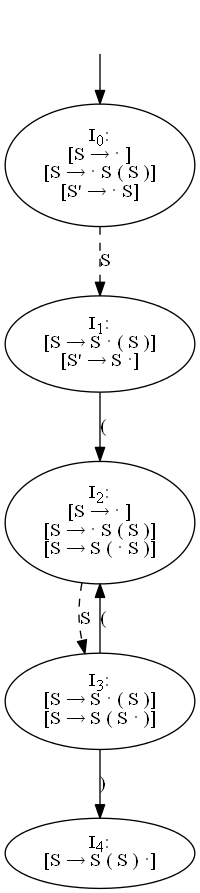
\includegraphics[scale=0.35]{examples/exampleLR0M.png}
	\centering
    \caption{LR(0) of examples/example.gra}
    \label{lrmex}
\end{figure}

\begin{table}[H]
    \begin{tabular}{| c | c | c | c || c |}
  \hline
  State & ( & ) & \$  & S \\ \hline
  I$_{0}$ & \shortstack{reduce S $\rightarrow$  $\epsilon$} & \shortstack{reduce S $\rightarrow$  $\epsilon$} & \shortstack{reduce S $\rightarrow$  $\epsilon$} & \shortstack{I$_{1}$} \\ \hline
  I$_{1}$ & \shortstack{shift I$_{2}$} & \shortstack{} & \shortstack{reduce S' $\rightarrow$  S} & \shortstack{} \\ \hline
  I$_{2}$ & \shortstack{reduce S $\rightarrow$  $\epsilon$} & \shortstack{reduce S $\rightarrow$  $\epsilon$} & \shortstack{reduce S $\rightarrow$  $\epsilon$} & \shortstack{I$_{3}$} \\ \hline
  I$_{3}$ & \shortstack{shift I$_{2}$} & \shortstack{shift I$_{4}$} & \shortstack{} & \shortstack{} \\ \hline
  I$_{4}$ & \shortstack{reduce S $\rightarrow$  S ( S )} & \shortstack{reduce S $\rightarrow$  S ( S )} & \shortstack{reduce S $\rightarrow$  S ( S )} & \shortstack{} \\ \hline
\end{tabular}

	\centering
    \caption{SLR(1) of examples/example.gra}
    \label{slrex}
\end{table}

Lastly let's generate the tiny LR(1) state machine along with the labels table:
\begin{lstlisting}[frame=single]
java -jar PTG.jar examples/example.gra -LR1M tiny tikz
\end{lstlisting}


\begin{figure}[H]
    \centering
	\begin{tabular}{l r}
        \begin{minipage}{2in}
			\begin{tikzpicture}[>=stealth',shorten >=1pt,auto,node distance=2cm,every text node part/.style={align=center}]
  \node[initial,state]  (i0)  {$I_0$};
  \node[state]  (i1)  [below of=i0]  {$I_{1}$};
  \node[state]  (i2)  [below of=i1]  {$I_{2}$};
  \node[state]  (i3)  [below of=i2]  {$I_{3}$};
  \node[state]  (i4)  [below of=i3]  {$I_{4}$};
  \node[state]  (i5)  [right of=i4]  {$I_{5}$};
  \node[state]  (i6)  [below of=i4]  {$I_{6}$};
  \node[state]  (i7)  [below of=i6]  {$I_{7}$};
  \path[->,dashed] (i0) edge [right] node {S} (i1);
  \path[->] (i1) edge [right] node {(} (i2);
  \path[->,dashed] (i2) edge [right] node {S} (i3);
  \path[->] (i3) edge [right] node {(} (i4);
  \path[->] (i3) edge [right] node {)} (i5);
  \path[->,dashed] (i4) edge [right] node {S} (i6);
  \path[->] (i6) edge [bend left] node {(} (i4);
  \path[->] (i6) edge [right] node {)} (i7);
\end{tikzpicture}

		\end{minipage}
		\begin{minipage}{2in}
			\begin{tabular}{| c | c |}
  \hline
  State & Current Rule Set \\ \hline
  I$_{0}$ & \shortstack{S $\rightarrow$  $\cdot$ $\epsilon$, \$  \\ S $\rightarrow$  $\cdot$ $\epsilon$, ( \\ S $\rightarrow$  $\cdot$ S ( S ), \$  \\ S $\rightarrow$  $\cdot$ S ( S ), ( \\ S' $\rightarrow$  $\cdot$ S, \$ } \\ \hline
  I$_{1}$ & \shortstack{S $\rightarrow$  S $\cdot$ ( S ), \$  \\ S $\rightarrow$  S $\cdot$ ( S ), ( \\ S' $\rightarrow$  S $\cdot$ , \$ } \\ \hline
  I$_{2}$ & \shortstack{S $\rightarrow$  $\cdot$ $\epsilon$, ( \\ S $\rightarrow$  $\cdot$ $\epsilon$, ) \\ S $\rightarrow$  $\cdot$ S ( S ), ( \\ S $\rightarrow$  $\cdot$ S ( S ), ) \\ S $\rightarrow$  S ( $\cdot$ S ), \$  \\ S $\rightarrow$  S ( $\cdot$ S ), (} \\ \hline
  I$_{3}$ & \shortstack{S $\rightarrow$  S $\cdot$ ( S ), ( \\ S $\rightarrow$  S $\cdot$ ( S ), ) \\ S $\rightarrow$  S ( S $\cdot$ ), \$  \\ S $\rightarrow$  S ( S $\cdot$ ), (} \\ \hline
  I$_{4}$ & \shortstack{S $\rightarrow$  $\cdot$ $\epsilon$, ( \\ S $\rightarrow$  $\cdot$ $\epsilon$, ) \\ S $\rightarrow$  $\cdot$ S ( S ), ( \\ S $\rightarrow$  $\cdot$ S ( S ), ) \\ S $\rightarrow$  S ( $\cdot$ S ), ( \\ S $\rightarrow$  S ( $\cdot$ S ), )} \\ \hline
  I$_{5}$ & \shortstack{S $\rightarrow$  S ( S ) $\cdot$ , \$  \\ S $\rightarrow$  S ( S ) $\cdot$ , (} \\ \hline
  I$_{6}$ & \shortstack{S $\rightarrow$  S $\cdot$ ( S ), ( \\ S $\rightarrow$  S $\cdot$ ( S ), ) \\ S $\rightarrow$  S ( S $\cdot$ ), ( \\ S $\rightarrow$  S ( S $\cdot$ ), )} \\ \hline
  I$_{7}$ & \shortstack{S $\rightarrow$  S ( S ) $\cdot$ , ( \\ S $\rightarrow$  S ( S ) $\cdot$ , )} \\ \hline
\end{tabular}

		\end{minipage}
    \end{tabular}
    \caption{LR(0) statemachine for examples/example.gra with tiny states along with labels table.}
    \label{lrex}
\end{figure}


To end this example, the full \LaTeX{} source file can be read in doc/UserManual.tex in the \href{https://github.com/EgillEinarss/PTG}{PTG repository}.

\end{document}